\documentclass{amsart}
\usepackage{tikz-cd}
\usepackage[bookmarks=true, linktocpage=true,
bookmarksnumbered=true, breaklinks=true,
pdfstartview=FitH, hyperfigures=false,
plainpages=false, naturalnames=true,
colorlinks=true, pagebackref=true,
pdfpagelabels]{hyperref}
\hypersetup{
	colorlinks,
	citecolor=blue,
	filecolor=blue,
	linkcolor=blue,
	urlcolor=blue
}

\renewcommand{\S}{\mathrm S}
\newcommand{\comch}{\texttt{ComCH}}
\newcommand{\id}{\mathrm{id}}
\newcommand{\X}{\mathcal X}

\begin{document}
\title[A C.A.S. for the study of commutativity up-to-coherent-homotopies]{A computer algebra system for the study of commutativity up-to-coherent-homotopies}
\author{Anibal M. Medina-Mardones}
\address{Max Plank Institute for Mathematics, Bonn, Germany}
\email{ammedmar@mpim-bonn.mpg.de}
\address{Department of Mathematics, University of Notre Dame, Notre Dame, IN, USA}
\email{amedinam@nd.edu}
\thanks{A.M-M. acknowledges financial support from Innosuisse grant \mbox{32875.1 IP-ICT - 1}, and the hospitality of the Max Plank Institute for Mathematics.}
\keywords{Computer algebra system, Python, homotopical algebra, operads, cohomology operations, cup product}

\begin{abstract}
	The Python package \comch\, is a lightweight specialized computer algebra system. It provides models for well known objects, the surjection and Barratt-Eccles operads, parameterizing the (co)product structure of (co)algebras that are (co)commutative in a derived sense. The primary example treated by \comch\, of these (co)algebras is the (co)chain complex of a space.
\end{abstract} 

\maketitle

\section{Introduction}

All the basic notions of number, from the integers to the complex, are equipped with a commutative product, and it was believed until Hamilton's introduction of the quaternions, that the product of any number system must be commutative. Hamilton's discovery encourage the consideration of other algebraic structures where commutativity was not demanded, and the conceptual shift that followed is only comparable to the effect non-euclidean geometries had in the study of spaces. Around a century later, after the development of the novel fields of topology and homotopy, mathematicians returned to the question of commutativity and identified additional levels of this property enriching the basic dichotomy. These structures correspond to coherent systems correcting homotopically the lack of strict commutativity, and constitute the focus of extensive current research in theoretical and applied topology. We mention knot theory, TQFT's, persistence homology and motion planning as some examples.

After the pioneering work of Steenrod \cite{Steenrod47, Steenrod62}, Adem \cite{Adem52}, Serre \cite{Serre53}, Cartan \cite{Cartan55}, Araki-Kudo \cite{ArakiKudo56}, Dyer-Lashof \cite{DyerLashof62}, Stashef \cite{Stasheff63}, Boardman-Vogt \cite{BoardmanVogt73}, May \cite{May70algebraic, May72geometry}, and many others, today there is a rich theory of commutativity up-to-coherent-homotopies whose modern framework is provided by operads and PROPs, and where $E_n$-operads play a central role parameterizing the different levels of homotopical commutativity. In \comch, we focus on the category of differential graded modules, and consider two models of the $E_\infty$-operad equipped with filtrations by $E_n$-operads. These are respectively due to McClure-Smith \cite{McClureSmith03} and Berger-Fresse \cite{BergerFresse04} and are known as the surjection and Barratt-Eccles operads.

The homology of algebras over $E_n$-operads are not only equipped with an induced commutative product but also, when the coefficient ring is the field $\mathbb F_p = \mathbb Z/ p\mathbb Z$, with homology operations. The study of these operations at the chain level has become an important issue in topological data analysis \cite{medina2018persistence}, condensed matter physics \cite{kapustin2017fermionic}, category theory \cite{medina2020globular} and others areas, and to provide researchers with effective tools for their study, \comch\, implements the constructions of \cite{medina2020chain}, making available for the first time chain level representations of these invariants for spaces presented simplicially or cubically.

\section*{Acknowledgment}
We gratefully acknowledge contributions from Djian Post, Wojciech Reise and Michelle Smith, stimulating conversations with Dennis Sullivan, Kathryn Hess, Greg Brumfiel, John Morgan, Ralph Kaufmann, Paolo Salvatore, Umberto Lupo, and Guillaume Tauzin, and the support of the Laboratory for Topology and Neuroscience at EPFL.

\section{Overview of \comch}

In this section we describe the overall structure and main functionalities of \comch, refering to its documentation for a complete description of all its classes and their methods.\footnote{Currently hosted at \url{https://comch.readthedocs.io/en/latest/}}

\subsection{Free modules and symmetric groups}

Let $R$ be the ring of integers or one of its quotients. In \comch\, the class \texttt{FreeModuleElement} serves to model elements in free $R$-modules, where $R$ is specified by the attribute \texttt{torsion}. Let $\S_r$ be the set of self-bijection of $\{1, \dots, r\}$ regarded as a group by composition. An element $\sigma \in \S_r$ will be represented by the sequence of its values $(\sigma(1), \dots, \sigma(r))$ and it is modeled in \comch\, using the class \texttt{SymmetricGroupElement}.

\subsection{Operads}

Operads parameterize algebraic structures on chain complexes. The precise although lengthy definition can be found for example in \cite{Markl08}. We will present a key example from which the definition can be abstracted. Let $C$ be a chain complex of $R$-module, and consider the set $End^C(r) = Hom(C, C^{\otimes r})$ of $R$-linear maps as a chain complex in the usual way. The set 
\begin{equation*}
End^C = \left\{End^C(r)\right\}_{r \geq 1}
\end{equation*}
is equipped with the following structure: a left action of $\S_r$ on $End^C(r)$ and composition chain maps
\begin{equation*}
\begin{tikzcd}[column sep=small, row sep=tiny]
\circ_i \colon &[-10pt] End^C(r) \otimes End^C(s) \arrow[r] & End^C(r+s-1) \\
& f \otimes g \arrow[r, |->] & (\id \otimes \cdots \otimes g \otimes \cdots \otimes \id) \circ f 
\end{tikzcd}
\end{equation*}
satisfying forms of equivariance, associativity, and unitality.

An $\mathcal O$-coalgebra structure on $C$ is a structure preserving morphism from $\mathcal O$ to $End^C$. We remark that it is also common to consider the operad $End_A$ obtained from the complexes $End_A(r) = Hom(A^{\otimes r}, A)$, referring to morphisms $\mathcal O \to End_A$ as $\mathcal O$-algebras. The linear duality functor induces from an $\mathcal O$-coalgebra in $C$ an $\mathcal O$-algebra structure on $Hom(C, R)$. In subsection \ref{label} we will overview the example given by (co)chains of simplicial sets.

\subsection{The symmetric ring operad}

Let us consider $R[\S] = \left\{R[\S_r]\right\}_{r \geq 1}$ with $R[\S_r]$ the group ring of $\S_r$ thought of as a dg $R$-module concentrated in degree~$0$. It has the structure of an operad with left action induced from left multiplication, and compositions induced from the maps
\begin{equation} \label{eq: compostion of permutations}
\circ_i \colon \S_r \times \S_s \to \S_{r+s-1}
\end{equation}
sending a pair $(x, y)$ to the bijection $x \circ_i y$ represented diagrammatically by
\begin{equation*}
\underbrace{1 \cdots (\overbrace{i \cdots i+s-1}^y) \cdots r+s-1}_x.
\end{equation*}
More precisely, $x \circ_i y$ is the sequence obtained by replacing the $i$-th value of $x$ with the sequence obtained by adding $i-1$ to the values of $y$, and shifting up by $s-1$ the values of $x$ greater than $s$. 

We model elements in $R[\S]$ using the class \texttt{SymmetricRingElement} which combines the classes \texttt{FreeModuleElement} and \texttt{SymmetricGroupElement}. For example, we have
\begin{verbatim}
>>> x = SymmetricRingElement({(2,3,1): -1, (1,3,2): 1})
>>> y = SymmetricRingElement({(1,3,2): 1, (1,2,3): 2})
>>> print(x * y)
- (2,1,3) - 2(2,3,1) + (1,2,3) + 2(1,3,2)
>>> print(x.compose(y, 2))
- (2,4,3,5,1) - 2(2,3,4,5,1) + (1,5,2,4,3) + 2(1,5,2,3,4)
\end{verbatim}

\subsection{$E_\infty$-operads}

An important class of operads are those defining resolutions of the ground ring $R$ as an $R[\S_r]$-module. Such operads are called \mbox{$E_\infty$-operads}. They typically come equipped with a filtration by so called $E_n$-operads parameterizing different levels of derived commutativity, with $E_1$ corresponding to the lack of any assumed commutativity, and $E_\infty$ to the largest possible degree of homotopical commutativity. \comch\, implements models of two well known $E_\infty$-operads equipped with filtrations by $E_n$-operads which we now describe.

\subsection{Surjection operad}

For a positive integer $r$ let $\mathcal X(r)_d$ be the free $R$-module generated by all functions $x : \{1, \dots, d+r\} \to \{1, \dots, r\}$ modulo the $R$-submodule generated by degenerate functions, i.e., those which are either non-surjective or have a pair of equal consecutive values. There is a left action of $\mathrm S_r$ on $\mathcal X(r)$ which is up to signs defined on basis elements by $\pi \cdot x = \pi \circ x$.
We represent a surjection $x$ as the sequences of its values $\big( x(1), \dots, x(n+r) \big)$. The boundary map in this complex is defined up to signs by
\begin{equation*}
\partial x = \sum_{i = 1}^{r+d} \pm \big( x(1), \dots, \widehat{x(i)}, \dots, x(n+r) \big),
\end{equation*}
and the $i$-th composition $x \circ_i y$ of $x \in \mathcal X(r)$ and $y \in \mathcal X(s)$ by the following. Let $w$ be the cardinality of $x^{-1}(i)$. For every collection of \textit{ordered indices}
\begin{equation*}
1 = j_0 \leq j_1 \leq j_2 \leq \cdots \leq j_{w-1} \leq j_w = s
\end{equation*}
we construct an associated splitting of $y$
\begin{equation*}
(y(j_0), \dots, y(j_1));\ (y(j_1), \dots, y(j_2));\ \cdots \ ;\ (y(j_{w-1}), \dots, y(j_w)).
\end{equation*}
The element $x \circ_i y \in \X(r+s-1)$ is represented, up to signs, as the sum over all possible collections of order indices of the sequence obtained in the following three steps: 1) shift up by $s-1$ the values of $x$ greater than $i$, then 2) shift up by $i-1$ the values of each sequence in the associated splitting of $y$, and finally 3) replace in order the occurrences of $i$ in $x$ by the corresponding sequence in the splitting.

The elements in this operad are modeled using the class \texttt{SurjectionElement}. For example,
\begin{verbatim}
>>> x = SurjectionElement({(1,2,1,3): 1})
>>> print(x.boundary())
(2,1,3) - (1,2,3)
>>> y = SurjectionElement({(1,2,1): 1})
>>> print({x.compose(y, 1))
(1,3,1,2,1,4) - (1,2,3,2,1,4) - (1,2,1,3,1,4)
\end{verbatim}

The signs appearing in these constructions are determined by the attribute \texttt{convention} with possible values the strings \texttt{McClure-Smith} and \texttt{Berger-Fresse}. We refer to \cite{McClureSmith03} and \cite{BergerFresse04} for details.

We will now review the definition of the complexity of a surjection element. The importance of this concept is that the set of surjection elements with complexity less than $n$ defines an $E_n$-suboperad of $\mathcal X$ \cite{McClureSmith03}.

The complexity of a finite binary sequence (i.e. a sequence of two distinct values) is defined as the number of consecutive distinct elements in it. For example, (1,2,2,1) and (1,1,1,2) have complexities 2 and 1 respectively. The complexity of a basis surjection element is defined as the maximum value of the complexities of its binary subsequences. Notice that for elements in $\mathcal X(2)$, complexity and degree agree. The class \texttt{SurjectionElement} models this concept with the attribute \texttt{complexity}.

\begin{verbatim}
>>> x = SurjectionElement({(1,2,1,3,1): 1})
>>> print(x.complexity)
1
\end{verbatim}

\subsection{Barratt-Eccles operad}

For a non-negative integer $r$ define the simplicial set $E(\mathrm S_r)$ by
\begin{align*}
E(\mathrm S_r)_n &= \{ (\sigma_0, \dots, \sigma_n)\ |\ \sigma_i \in \mathrm{S}_r\}, \\
d_i(\sigma_0, \dots, \sigma_n) &= (\sigma_0, \dots, \widehat{\sigma}_i, \dots, \sigma_n), \\
s_i(\sigma_0, \dots, \sigma_n) &= (\sigma_0, \dots, \sigma_i, \sigma_i, \dots, \sigma_n).
\end{align*}
It is equipped with a left $\mathrm S_r$-action defined on basis elements by
\begin{equation*}
\sigma (\sigma_0, \dots, \sigma_n) = (\sigma \sigma_0, \dots, \sigma \sigma_n).
\end{equation*}
The chain complex resulting from applying the functor of normalized $R$-chains to it is denoted $\mathcal E(r)$ and the underlying set of the Barratt-Eccles operad is $\mathcal E = \{\mathcal E(r)\}_{r\geq0}$. To define its composition structure we use the Eilenberg-Zilber map. Let us notice that at the level of the simplicial sets $E(\S_r)$ we have compositions
\begin{equation*}
{\circ}_{i}: E(r) \times E(s) \to E(r + s - 1)
\end{equation*}
induced coordinate-wise from $\eqref{eq: compostion of permutations}$.
We define the composition of $\mathcal E$ by precomposing
\begin{equation*}
N_\bullet(\circ_i) \colon N_\bullet(E(r) \times E(s))
\longrightarrow
N_\bullet(E(r + s - 1)) = \mathcal E(r+s-1)
\end{equation*}
with the iterated Eilenberg-Zilber map
\begin{equation*}
\mathcal E(r) \otimes \mathcal E(s) =
N_\bullet(E(r)) \otimes N_\bullet(E(s))
\longrightarrow
N_\bullet(E(r) \times E(s)).
\end{equation*}
For example,
\begin{verbatim}
>>> x = BarrattEcclesElement({((1,2),(2,1)):1, ((2,1),(1,2)):2})
>>> print(x.boundary())
((1,2),) - ((2,1),)
>>> y = BarrattEcclesElement({((2,1,3),):3})
>>> print(x.compose(y, 2))
3((1,3,2,4),(3,2,4,1)) + 6((3,2,4,1),(1,3,2,4))
\end{verbatim}

The complexity of a Barratt-Eccles element is define analogously to that of surjection elements. In this case too, the subset of elements with complexity less than $n$ defines an $E_n$-suboperad \cite{BergerFresse04}.

An important structure present in the Barratt-Eccles operad missing in the surjection operad is a diagonal chain map compatible with compositions. It is the Alexander-Whitney diagonal defined on basis Barratt-Eccles element by
\begin{equation*}
\Delta(\sigma_0, \dots, \sigma_n) = \sum_{i=1}^n (\sigma_0, \dots, \sigma_i) \otimes (\sigma_i, \dots, \sigma_n).
\end{equation*}
We illustrate its implmentation in \comch\, with the following example.
\begin{verbatim}
>>> x = BarrattEcclesElement({((1,2), (2,1)): 1})
>>> print(x.diagonal())
(((1, 2),), ((1, 2), (2, 1))) + (((1, 2), (2, 1)), ((2, 1),))
\end{verbatim}

\section{Steenrod operations}

\subsection{Steenrod-Adem structures}

Let $\mathrm{C}_r$ be the cyclic group of order $r$ thought of as the subgroup of $\mathrm{S}_r$ generated by an element $\rho$. The elements
\begin{equation*}
T = \rho-1 \quad \text{ and } \quad N = 1+\rho+\cdots+\rho^{r-1}
\end{equation*}
in $R[C_r]$ define a minimal resolution $W(r)$
\begin{equation*}
R[C_r] \stackrel{T}{\longleftarrow} R[C_r] \stackrel{N}{\longleftarrow} R[C_r] \stackrel{T}{\longleftarrow} \cdots
\end{equation*}
of $R$ by free $R[C_r]$-modules. We denote
a preferred basis element of $W(r)_i$ by $e_i$.

A Steenrod-Adem structure on an operad $\mathcal O$ is a collection of $\mathrm C$-equivariant chain maps $\mathcal W \stackrel{\psi}{\longrightarrow} \mathcal O$ for which there exists a factorization through an $E_\infty$-operad $\mathcal W \stackrel{\iota}{\longrightarrow} \mathcal R \stackrel{\phi}{\longrightarrow} \mathcal O$ such that $\iota$ is a weak equivalence and $\phi$ a morphism of operads. For any integers $r$ and $i$, a Steenrod-Adem structure produces a preferred element $\psi(e_i)$ in $\mathcal O(r)_i$. 

Steenrod-Adem structures for the surjection and Barratt-Eccles operads are implemented in \comch\, following their introduction in \cite{medina2020chain}. For example,

\begin{verbatim}
>>> r, i = 3, 2
>>> x = BarrattEccles.steenrod_adem_structure(r, i)
>>> print(x)
((1,2,3),(2,3,1),(3,1,2)) + ((1,2,3),(3,1,2),(1,2,3))
>>> y = Surjection.steenrod_adem_structure(r, i)
>>> print(y)
(1,2,3,1,2) + (1,3,1,2,3) + (1,2,3,2,3)
\end{verbatim}

\subsection{Interpreting surjections as linear maps}

To connect with the theory of Steenrod operations on the cohomology of spaces, we need to describe how to interpret a surjection as an element in $Hom(C_\bullet, C_\bullet^{\otimes r})$. We use the diagrammatical language and constructions of \cite{medina2020prop1, medina2018prop2}. Represent a basis surjection element in $\mathcal X(r)_n$ as the labeled directed graph
\begin{center}
	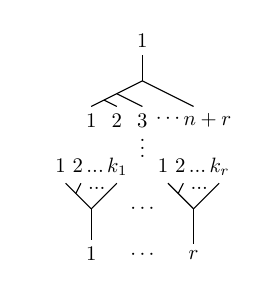
\begin{tikzpicture}[scale=.65]
	\draw (0,0)--(0,-.6) node[below, scale=.75]{$1$};
	\draw (0,0)--(.5,.5);
	\draw (-.3, .3)-- (-.2,.5) node[above, scale=.75]{\quad $1\ 2\, ...\, k_1$};
	\draw (-.5,.5)--(0,0);
	\node[scale=.75] at (.11,.4){$...$};
	
	\node[scale=.75] at (1,0){$\cdots$};
	\node[scale=.75] at (1,-.9){$\cdots$};
	
	\draw (2,0)--(2,-.68) node[scale=.75, below]{$r$};
	\draw (2,0)--(2.5,.5);
	\draw (1.7, .3)-- (1.8,.5) node[scale=.75, above]{\quad $1\ 2\, ...\, k_r$};
	\draw (1.5,.5)--(2,0);
	\node[scale=.75] at (2.11,.4){$...$};
	
	\draw (1,2.5)--(1,3) node[scale=.75, above]{$1$};
	\draw (1,2.5)--(0,2) node[scale=.75, below]{$1$};
	\draw (.25,2.125)--(.5,2) node[scale=.75, below]{$2$};
	\draw (.5,2.25)--(1,2) node[scale=.75, below]{$3$};
	\draw (1,2.5)--(2,2) node[scale=.75, below]{\ \quad $n + r$};
	\node[scale=.75] at (1.5,1.75){$\cdots$};
	
	\node[scale=.75] at (1,1.3) {$\vdots$};
	
	\node at (2.85,0){};
	\end{tikzpicture}
\end{center}
where there are no hidden vertices and the strands at the top are joined to the strands in the bottom using the surjection. Any such graph gives rise to a map in $Hom(C_\bullet, C_\bullet^{\otimes r})$ after associating maps to the generating pieces
\begin{tikzpicture}[scale=.25]
\draw (0,.5)--(0,1.25);
\draw (0,.5)--(.5,0);
\draw (0,.5)--(-.5,0);
\end{tikzpicture}
and
\begin{tikzpicture}[scale=.25]
\draw (0,.75)--(0,0);
\draw (0,.75)--(.5,1.25);
\draw (0,.75)--(-.5,1.25);
\end{tikzpicture}
in $Hom(C_\bullet, C_\bullet^{\otimes 2})$ and $Hom(C_\bullet^{\otimes 2}, C_\bullet)$ respectively. As explained in \cite{medina2020chain}, this can be done when $C_\bullet$ is either the chains on a standard simplex or a standard cube, in manner such that the resulting linear map $\X(r) \to Hom(C_\bullet, C_\bullet^{\otimes r})$ is a chain map.

In \comch\, we implement models for $C_\bullet^{\otimes r}$ and describe the action of a surjection element. For example,
\begin{verbatim}
>>> x = SurjectionElement({(1, 2, 1): 1}, convention='McClure-Smith')
>>> simplex = Simplicial.standard_element(2)
>>> print(x(simplex))
- ((0,1,2),(0,1)) + ((0,2),(0,1,2)) - ((0,1,2),(1,2))
>>> cube = Cubical.standard_element(2)
>>> print(x(cube))
- ((2,2),(1,2)) + ((2,1),(2,2)) + ((0,2),(2,2)) - ((2,2),(2,0))
\end{verbatim}

\bibliographystyle{ieeetr}
\bibliography{bibliography}

\end{document}